\chapter{Methodology}
The implementation methodology consists of three distinct phases: setting up a local LLM agent with Ollama, configuring a multi-agent collaboration workflow using CrewAI, and designing a production-grade sequential agent pipeline in n8n. The integration of mathematical calculator tools with language models is key to resolving mathematical inaccuracies (hallucinations) common in deep learning models.

\section{Write Agent using Ollama}
The foundation of our system is the deployment of local Large Language Models (LLMs) on consumer-grade hardware. Ollama serves as a local inference runner, hosting the Llama 3.2 3B parameter model and exposing a standardized API endpoint on port 11434. 

To build an agent, we write Python wrappers that interface with this endpoint, handling variable formatting and system prompts. Prompt engineering is used to control output style and temperature. Listing \ref{lst:ollama_agent} shows a Python wrapper for generating structured single-agent queries.

\begin{lstlisting}[language=Python, caption=Python Implementation of Local Ollama Agent, label=lst:ollama_agent]
import urllib.request
import json

class LocalOllamaAgent:
    def __init__(self, model_name="llama3.2", base_url="http://localhost:11434"):
        self.model_name = model_name
        self.base_url = f"{base_url}/api/generate"

    def invoke(self, system_prompt, user_query):
        payload = {
            "model": self.model_name,
            "prompt": f"System: {system_prompt}\nUser: {user_query}\nResponse:",
            "stream": False,
            "options": {
                "temperature": 0.2
            }
        }
        
        req = urllib.request.Request(
            self.base_url,
            data=json.dumps(payload).encode("utf-8"),
            headers={"Content-Type": "application/json"}
        )
        
        try:
            with urllib.request.urlopen(req) as response:
                res_data = json.loads(response.read().decode("utf-8"))
                return res_data.get("response", "")
        except Exception as e:
            return f"Error connecting to Ollama: {str(e)}"

# Example usage
if __name__ == "__main__":
    agent = LocalOllamaAgent()
    sys_msg = "You are a budgeting expert. Format your reply in one line."
    reply = agent.invoke(sys_msg, "I earn 50000 and spend 30000. What is my savings rate?")
    print("Agent Response:", reply)
\end{lstlisting}

\section{Multi-agents with LangChain, CrewAI and Ollama}
While a single model handles basic text generation, multi-agent frameworks are required to model complex scenarios that require distinct personas, guidelines, and access to tools. The CrewAI framework is used to define role-playing agents, configure task assignments, and orchestrate collaboration. LangChain binds our local Ollama model to the CrewAI framework.

The agents execute tasks sequentially:
\begin{enumerate}
    \item \textbf{Budget Agent}: Analyzes the user query and runs the budgeting tool to calculate surpluses.
    \item \textbf{Investment Agent}: Formulates asset allocations using compounding projections.
    \item \textbf{Debt Agent}: Resolves EMI payment terms and payoff methods.
    \item \textbf{Tax Agent}: Evaluates regime efficiency (Old vs New).
\end{enumerate}

Listing \ref{lst:crewai_multiagent} details the implementation of a collaborative multi-agent financial advisor system in CrewAI.

\begin{lstlisting}[language=Python, caption=Multi-Agent Collaboration in CrewAI, label=lst:crewai_multiagent]
from crewai import Agent, Task, Crew, Process, LLM
from langchain.tools import tool

# Define local Ollama configuration via LangChain-compatible CrewAI LLM wrapper
local_llm = LLM(
    model="ollama/llama3.2:3b",
    base_url="http://localhost:11434"
)

@tool("budget_calculator")
def budget_calculator(monthly_income: float, monthly_expenses: float) -> str:
    """Calculates savings surplus and emergency fund target."""
    surplus = monthly_income - monthly_expenses
    emergency_fund = monthly_expenses * 6
    return f"Surplus: {surplus}, Emergency Target: {emergency_fund}"

# Define Agents
budget_agent = Agent(
    role="Budgeting Specialist",
    goal="Analyze cash flows and establish budget targets.",
    backstory="You evaluate spending behaviors and emergency preparedness.",
    tools=[budget_calculator],
    llm=local_llm,
    verbose=True
)

investment_agent = Agent(
    role="Investment Strategist",
    goal="Identify wealth-creation opportunities and run compounding plans.",
    backstory="Senior advisor focused on mutual funds, gold, and PPF allocations.",
    llm=local_llm,
    verbose=True
)

# Define Tasks
budget_task = Task(
    description="Analyze query: 'I earn 50000 and spend 30000.' Run the calculator.",
    expected_output="A structured report mapping surplus and emergency fund sizes.",
    agent=budget_agent
)

investment_task = Task(
    description="Develop compounding recommendations based on the budget analysis.",
    expected_output="An allocation plan showing long-term investment goals.",
    agent=investment_agent
)

# Assemble Crew
financial_crew = Crew(
    agents=[budget_agent, investment_agent],
    tasks=[budget_task, investment_task],
    process=Process.sequential
)

result = financial_crew.kickoff()
print("Crew Final Output:", result)
\end{lstlisting}

\section{Multi-agent using n8n and Ollama}
To build a production system, we deploy the multi-agent architecture in n8n. This platform provides visual debugging, webhook routing, database integrations, and JSON parsing tools. Figure \ref{fig:n8n_workflow} displays the visual multi-agent personal financial advisor workflow implemented in n8n.

\begin{figure}[H]
    \centering
    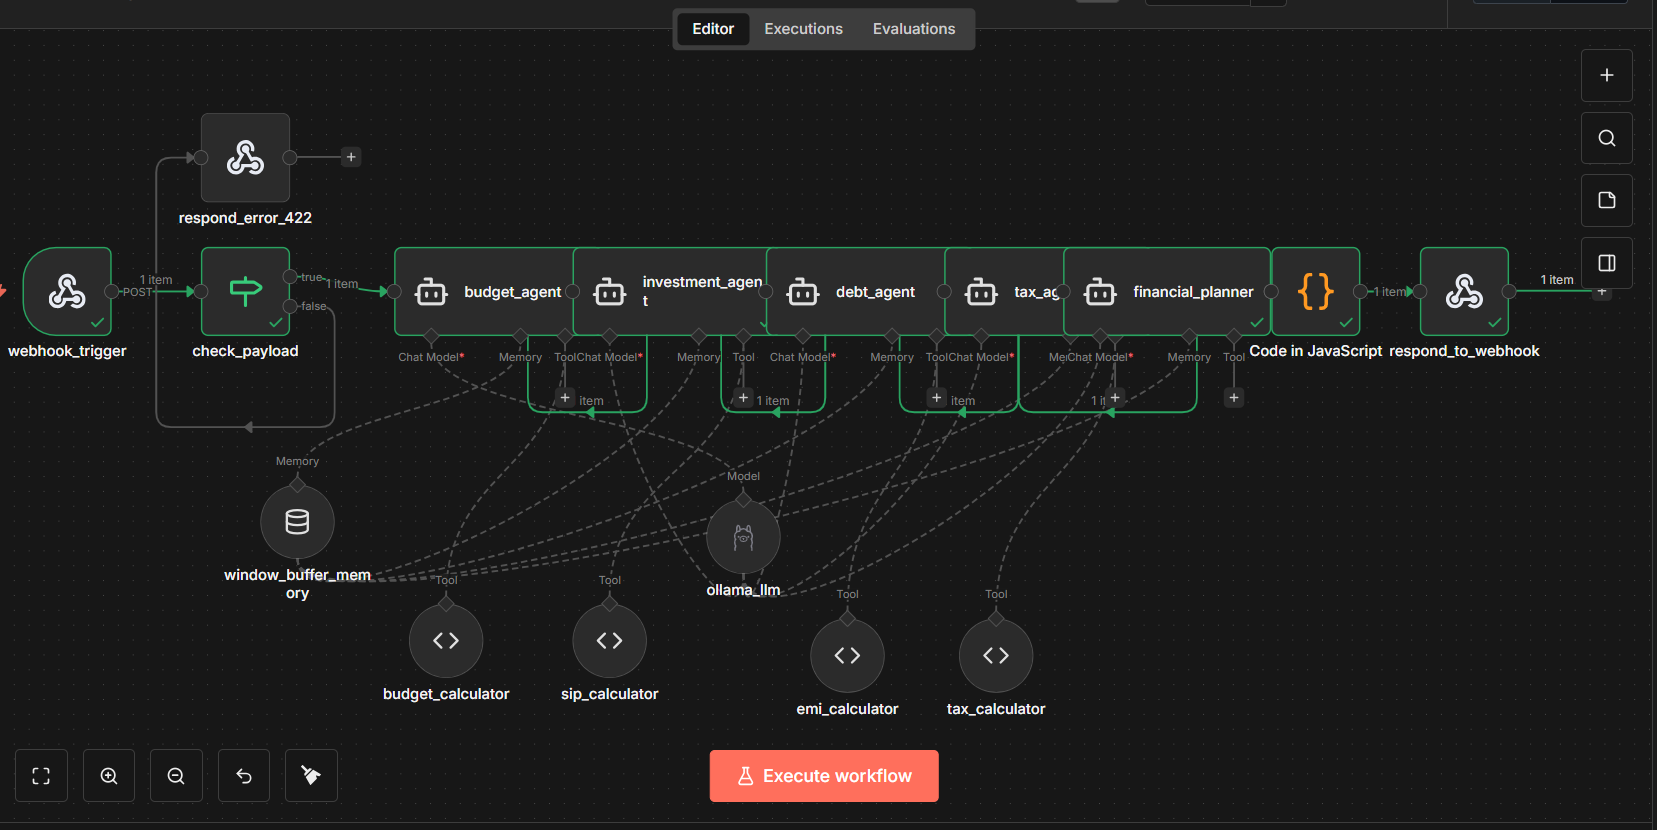
\includegraphics[width=0.95\textwidth]{images/n8n_Personal_Financial_Agent.png}
    \caption{Multi-Agent Workflow Implemented in n8n}
    \label{fig:n8n_workflow}
\end{figure}

The node execution flow operates as follows:
\begin{enumerate}
    \item \textbf{Trigger Node}: An HTTP POST Webhook node accepting parameters (\texttt{session\_id} and \texttt{message}) on the \texttt{/webhook/finance-advisor} endpoint.
    \item \textbf{Check Payload (IF Node)}: A validation node that verifies the presence of parameters.
    \item \textbf{Financial Analysis Agent (Budget Agent)}: Evaluates the query using the custom JS \texttt{budget\_calculator} tool.
    \item \textbf{Investment Agent}: Builds mutual fund and PPF recommendations using the JS \texttt{sip\_calculator} tool.
    \item \textbf{Loan Agent (Debt Agent)}: Formulates payment schedules using the JS \texttt{emi\_calculator} tool.
    \item \textbf{Tax Agent}: Calculates tax efficiency comparison using the JS \texttt{tax\_calculator} tool.
    \item \textbf{Report Generator Agent (Financial Planner)}: Combines all outputs into a single JSON object.
\end{enumerate}

To prevent validation crashes common to lightweight local models (which occasionally format numbers as strings), the custom JS tools are mapped to a relaxed schema: \texttt{["number", "string", "null"]}. Table \ref{table:tool_schemas} details the inputs accepted by these calculators.

\begin{table}[H]
    \centering
    \caption{Custom Tool Schemas}
    \label{table:tool_schemas}
    \begin{tabular}{lllp{6cm}}
        \toprule
        \textbf{Tool Name} & \textbf{Parameter} & \textbf{Type} & \textbf{Description} \\
        \midrule
        budget\_calculator & monthly\_income & [number, string, null] & Monthly earnings. \\
        & monthly\_expenses & [number, string, null] & Monthly expenditure. \\
        \midrule
        sip\_calculator & monthly\_investment & [number, string, null] & Monthly SIP contribution. \\
        & expected\_return\_rate & [number, string, null] & Annual yield rate. \\
        & years & [number, string, null] & Investment timeline in years. \\
        \midrule
        emi\_calculator & principal & [number, string, null] & Total loan principal. \\
        & annual\_interest\_rate & [number, string, null] & Annual loan rate percentage. \\
        & years & [number, string, null] & Repayment tenure in years. \\
        \midrule
        tax\_calculator & annual\_income & [number, string, null] & Total yearly taxable earnings. \\
        \bottomrule
    \end{tabular}
\end{table}

Each of the custom tools is implemented with deterministic mathematical algorithms to ground the language model's reasoning:
\begin{enumerate}
    \item \textbf{Budget Calculator}: Evaluates monthly surplus and savings rate. It projects the popular 50-30-20 budget allocation scheme (allocating 50\% of monthly income to core Needs, 30\% to optional Wants, and 20\% to Savings) and calculates a 6-month emergency reserve cushion based on monthly expenses.
    \item \textbf{SIP Calculator}: Simulates systematic monthly investment plans by executing the Future Value of an Annuity Due formula:
    \[
    FV = P \times \left( \frac{(1 + r)^n - 1}{r} \right) \times (1 + r)
    \]
    where $P$ is the monthly investment, $r$ is the monthly expected return rate, and $n$ is the total number of months. It outputs the total invested capital, final maturity value, and compound wealth gained over the tenure.
    \item \textbf{EMI Calculator}: Resolves loan amortization parameters. It executes the standard amortization formula to calculate the monthly payment:
    \[
    EMI = P \times \frac{r(1+r)^n}{(1+r)^n - 1}
    \]
    where $P$ is the loan principal, $r$ is the monthly interest rate, and $n$ is the total number of months. It calculates the total interest payable and repayment totals.
    \item \textbf{Tax Calculator}: Models yearly income tax obligations under the Indian Tax Slab rules. Under the New Regime (FY 2024-25), it deducts a standard deduction of INR 75,000 and calculates tax progressively (5\% for 3L--6L, 10\% for 6L--9L, 15\% for 9L--12L, 20\% for 12L--15L, and 30\% above 15L). Under the Old Regime, it applies standard deductions of INR 225,000 (INR 50,000 standard deduction + INR 150,000 Section 80C + INR 25,000 Section 80D) and computes tax at historical slab rates.
\end{enumerate}

Listing \ref{lst:js_sip_tool} shows the Javascript parser implemented inside the \texttt{sip\_calculator} node to handle unformatted inputs from the LLM.

\begin{lstlisting}[language=JavaScript, caption=JavaScript Implementation of the SIP Calculator Tool, label=lst:js_sip_tool]
try {
  let sip = null;
  let rate_annual = null;
  let years = null;
  
  if (query && typeof query === 'object') {
    sip = typeof query.monthly_investment === 'number' ? query.monthly_investment : (parseFloat(query.monthly_investment) || null);
    rate_annual = typeof query.expected_return_rate === 'number' ? query.expected_return_rate : (parseFloat(query.expected_return_rate) || null);
    years = typeof query.years === 'number' ? query.years : (parseInt(query.years) || null);
  }
  
  if (sip === null || rate_annual === null || years === null) {
    let text = '';
    if (typeof query === 'string') {
      text = query;
    } else if (query && typeof query === 'object') {
      text = query.query || query.input || '';
    }
    
    const parseNum = (matchResult) => {
      if (!matchResult) return null;
      let val = parseFloat(matchResult[1]);
      const unit = (matchResult[2] || '').toLowerCase();
      if (unit.startsWith('k')) val *= 1000;
      else if (unit.startsWith('l')) val *= 100000;
      else if (unit.startsWith('m')) val *= 1000000;
      return val;
    };
    
    if (sip === null) {
      sip = parseNum(text.match(/(?:sip|monthly|invest|saving)\D*(\d+(?:\.\d+)?)\s*(k|lakh|l|m)?/i));
    }
    if (rate_annual === null) {
      const pctMatch = text.match(/(\d+(?:\.\d+)?)\s*%/);
      if (pctMatch) {
        rate_annual = parseFloat(pctMatch[1]);
      } else {
        const rateMatch = text.match(/(?:rate|return|interest|yield)\D*(\d+(?:\.\d+)?)/i);
        if (rateMatch) rate_annual = parseFloat(rateMatch[1]);
      }
    }
    if (years === null) {
      const yrMatch = text.match(/(\d+)\s*(?:year|yr|y)/i);
      if (yrMatch) {
        years = parseInt(yrMatch[1]);
      } else {
        const yearsMatch = text.match(/(?:year|duration|time|period)\D*(\d+)/i);
        if (yearsMatch) years = parseInt(yearsMatch[1]);
      }
    }
  }
  
  if (sip === null || rate_annual === null || years === null) {
    return "Error: Missing required inputs for SIP calculation.";
  }
  
  const rate_monthly = rate_annual / 12 / 100;
  const months = years * 12;
  const total_invested = sip * months;
  const maturity_value = sip * ((Math.pow(1 + rate_monthly, months) - 1) / rate_monthly) * (1 + rate_monthly);
  const estimated_returns = maturity_value - total_invested;
  
  const fmt = (num) => num.toLocaleString('en-US', { minimumFractionDigits: 2, maximumFractionDigits: 2 });
  
  return `Monthly SIP: INR ${fmt(sip)}
Tenure: ${years} years
Expected Return Rate: ${rate_annual.toFixed(2)}%
Total Invested: INR ${fmt(total_invested)}
Maturity Value: INR ${fmt(maturity_value)}
Wealth Gained: INR ${fmt(estimated_returns)}`;
} catch (e) {
  return 'Error: ' + e.message;
}
\end{lstlisting}

\section{Results and Detailed Discussion}
The front-end user interface is implemented via Streamlit, allowing users to submit financial queries and view parsed JSON tabular reports. Figure \ref{fig:streamlit_ui} displays the financial advisor front-end interface.

\begin{figure}[H]
    \centering
    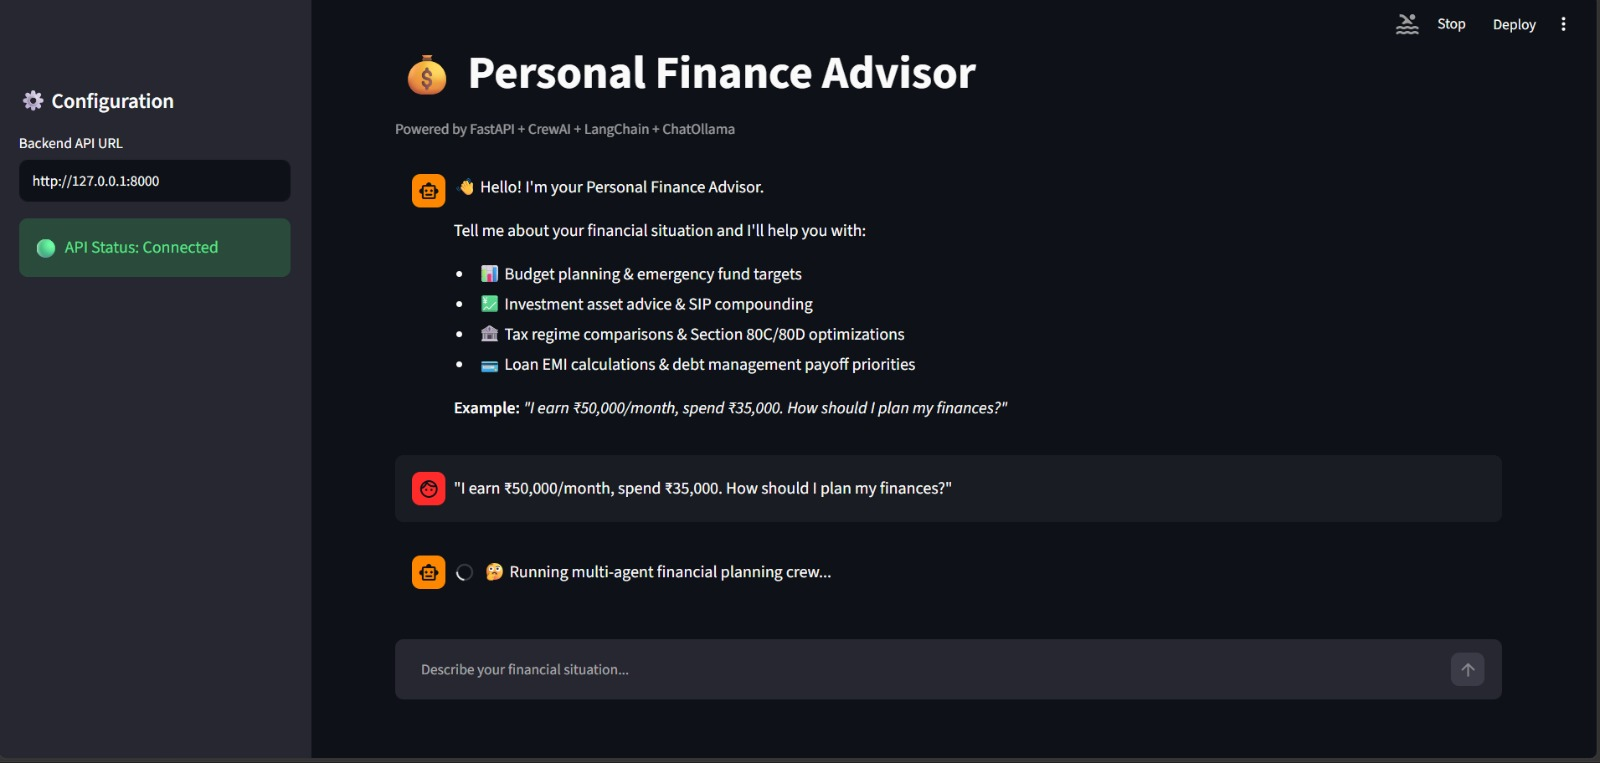
\includegraphics[width=0.95\textwidth]{images/Interface_Financial_Advisor.png}
    \caption{Financial Advisor User Interface}
    \label{fig:streamlit_ui}
\end{figure}

Upon executing the multi-agent n8n workflow, the financial planner agent parses and formats the outputs. Figure \ref{fig:output_screenshot} displays the generated client-ready financial advisory report.

\begin{figure}[H]
    \centering
    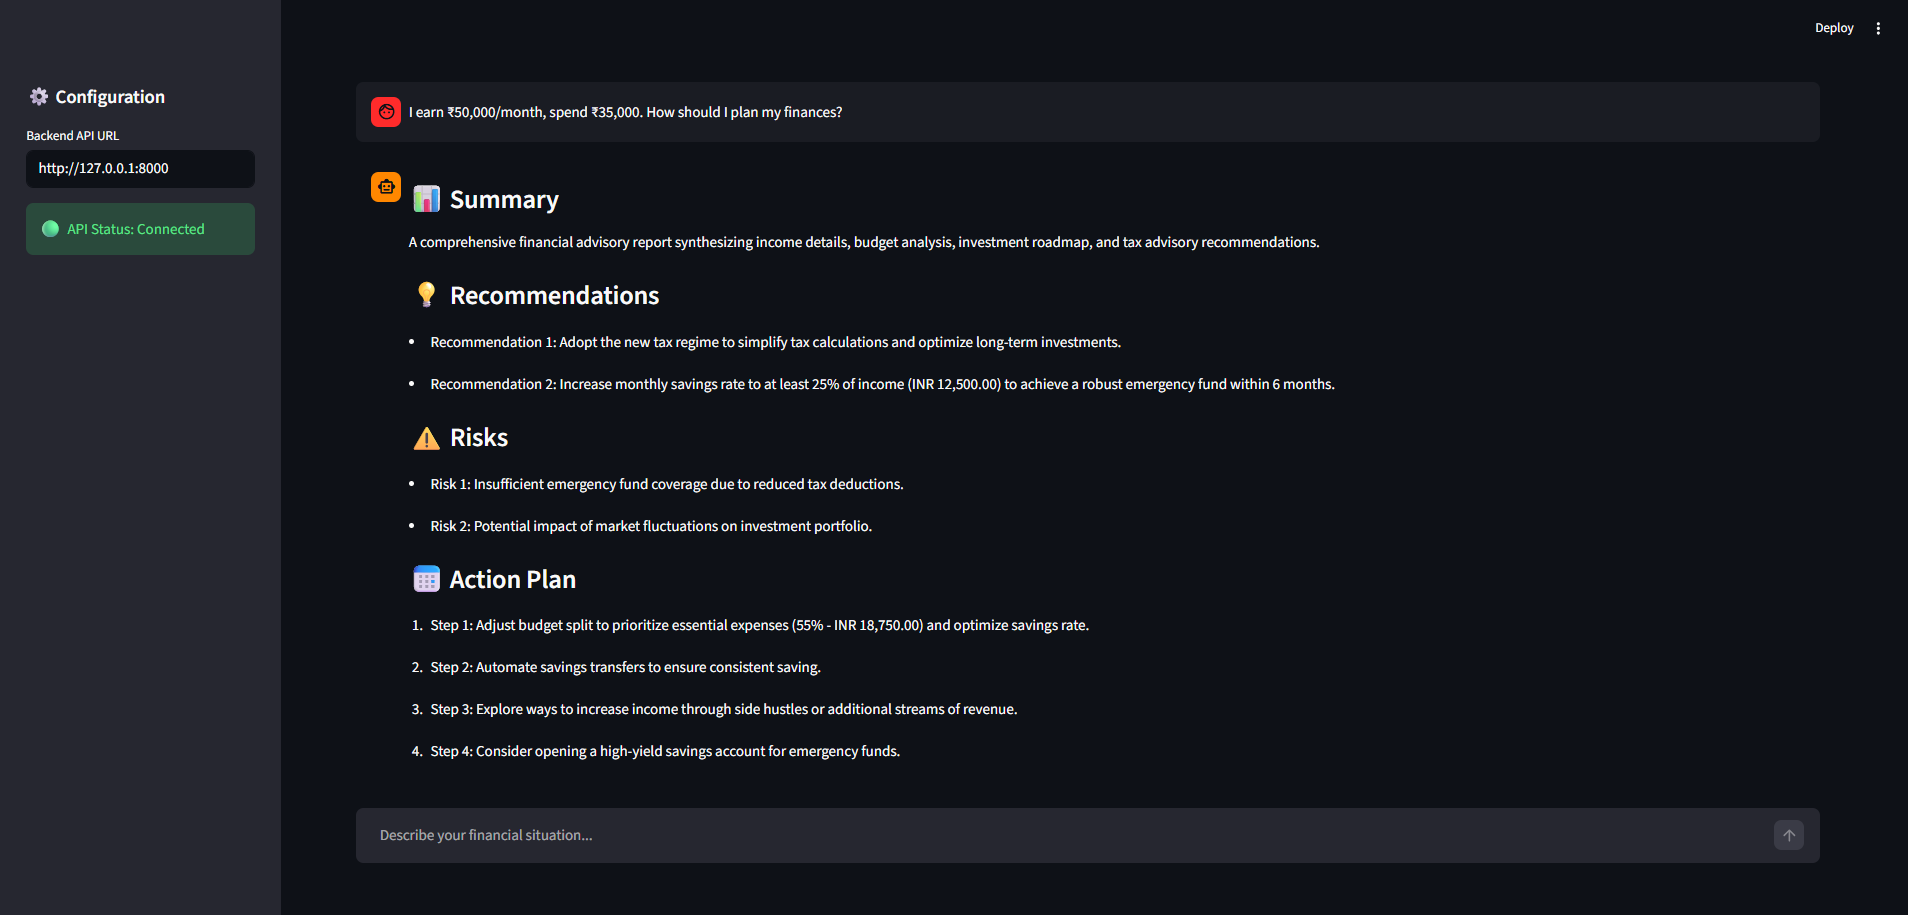
\includegraphics[width=0.95\textwidth]{images/Personal_Finance_Advisor.png} 
    \caption{Generated Financial Advisory Report}
    \label{fig:output_screenshot}
\end{figure}

The advisory output compiles recommendations, identifies financial risks (such as high expenditure rates or lack of retirement assets), and outlines an actionable step-by-step financial plan. The integration of custom calculators ensures that the LLM's natural language advice is grounded in verified, mathematical calculations. Listing \ref{lst:json_output} represents a sample JSON response returned by the system.

\begin{lstlisting}[language=json, caption=JSON Advisory Report Response, label=lst:json_output]
{
  "summary": "Calculated budget with 50-30-20 splits based on monthly income of INR 50,000.00 and expenses of INR 30,000.00. Investment parameters were missing and noted in the report.",
  "recommendations": [
    "Aim to invest your surplus of INR 20,000.00 to build long-term wealth.",
    "Allocate INR 25,000.00 to Needs, INR 15,000.00 to Wants, and INR 10,000.00 to Savings.",
    "Build a 6-month emergency fund target of INR 180,000.00."
  ],
  "risks": [
    "Your current savings rate is 40.00% which is good, but keeping surplus in cash risks inflation erosion.",
    "No investment, tax optimization, or debt data was supplied."
  ],
  "action_plan": [
    "Review your monthly expenses to find areas where you can reduce wants.",
    "Define your SIP goals and provide monthly investment details to run the SIP calculator.",
    "Establish your emergency fund in a liquid savings account."
  ]
}
\end{lstlisting}

This multi-agent sequential pipeline ensures that calculations from the Budget Agent are passed directly into the context of the Investment and Debt Agents, maintaining contextual alignment across all calculations.
